\section{Evaluation}\label{sec:eval}

\subsection{Methodology}\label{sec:eval:method}
\paragraph{Simulators}
All algorithms are implemented once, in a ROS-independent library that is executed both by a fast
multi-agent simulator and by the ROS~2 nodes running against PX4 SITL in Gazebo
(Section~\ref{sec:impl}). The fast simulator advances all UAVs with a 0.5\,s control step, samples
every broadcast through the channel model of Section~\ref{sec:model} (path loss, building
obstructions, correlated shadowing, Rician/Rayleigh fading, collision interference) and produces
detections with the calibrated sensing model. Each run starts from a procedurally generated
disaster area (tall buildings that are no-fly zones and obstruct links, low rubble that occludes
victims, warm debris that causes false alarms, 25 victims of which one is fully buried) and lasts
600\,s. Unless stated otherwise the area is 400\,m$\times$400\,m, $N=8$, the channel is
urban-rubble, and UAVs fail as a Poisson process with rate 0.01\,s$^{-1}$ per swarm.

\paragraph{Metrics}
The primary metric is the share of all victims whose report reaches the responder within 60\,s of
their first confirmation (\emph{reported $\le$60\,s}); its denominator is the number of victims in
the area, so a method cannot score well by detecting few. We also report the share of victims
reported by the end of the mission, the 90th-percentile report latency, coverage of the reachable
area, information loss (victims confirmed by some UAV whose every holder failed before the report
reached the responder), false confirmed entries, and the per-agent planning time.

\paragraph{Baselines}
B0: constriction PSO with the same exploration layer and no communication term; B1: the earlier SENTINEL design
(nearest-neighbour distance spring, $R=50$\,m); B2: communication-aware PSO with
a soft outage penalty on all neighbours; B3: algebraic-connectivity gradient control
\cite{sabattini2013} given the \emph{exact} $\lambda_2$ and Fiedler vector of the swarm at every step
(an oracle that favours B3); B4: edge-tension potential with hysteresis \cite{ji2007};
B5: MAPPO \cite{yu2022mappo} with a parameter-shared actor on local observations and a centralised
critic; B6: boustrophedon sweep of static sectors. All methods share sensing, gossip, the ledger and
the channel, so they differ only in how UAVs move.

\paragraph{Fair tuning and statistics}
Every method's free parameters were tuned with the same budget (Optuna TPE, 30 trials, each scored
on six runs in an urban $N=8$ and a severe $N=4$ scenario) on seeds 1000--1002, which are never used
for evaluation. MAPPO was trained for 600 PPO iterations of 16 episodes each (9\,600 missions) on
separate seeds and selected on the same tuning seeds; its training return plateaus after about 150
iterations (Fig.~\ref{fig:mappo}), so the reported policy is not limited by training length. Each
configuration is evaluated on seeds 0--29; all methods see the same area, victims and failure
schedule for a given seed (common random numbers). We report means with 95\,\% bootstrap
confidence intervals and test SENTINEL against every other method with paired Wilcoxon
signed-rank tests, Holm-corrected within each scenario (marked $^*$ in the tables for $p<0.05$).
In total the evaluation comprises about 11\,000 simulated missions.

\begin{figure}[t]\centering
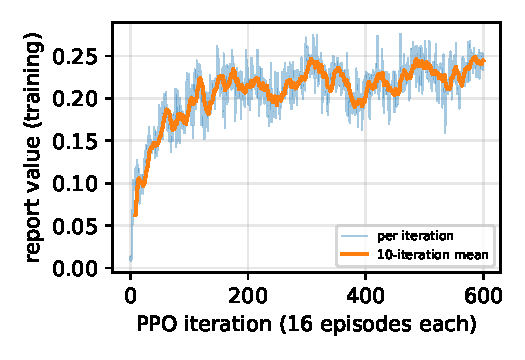
\includegraphics[width=\columnwidth]{figures/mappo_curve.pdf}
\caption{Training curve of the MAPPO baseline (B5): time-discounted report value per PPO iteration
and its 10-iteration mean. The return plateaus after about 150 iterations.}
\label{fig:mappo}
\end{figure}

\subsection{Onboard perception}\label{sec:eval:perception}
Table~\ref{tab:perception} compares YOLO26n with YOLOv8n trained under an identical protocol on
HIT-UAV \cite{hituav}. The two detectors reach the same mAP50 (0.948 vs.\ 0.947); YOLO26n is more
precise (0.932 vs.\ 0.909) and better localised (mAP50-95 0.533 vs.\ 0.520) with slightly lower
recall, and it needs 19\,\% fewer parameters and 31\,\% fewer operations. On a desktop GPU the two
are equally fast (about 1.8\,ms end-to-end with TensorRT FP16); we therefore attribute YOLO26n's
suitability for low-power hardware to its lower compute, not to measured speed, and we do not report
embedded latency, which was not measured. The accuracy values are the validation metrics recorded by
the training runs.
% generated by make_results.py -- do not edit by hand
\begin{table*}[t]\centering\caption{Thermal detectors trained with the same protocol (HIT-UAV, 100 epochs, AdamW, 640 px, seed 0). Accuracy: validation metrics recorded by the training run. Latency: end-to-end p50 on an RTX 3060 (desktop), PyTorch FP32 and TensorRT FP16.}\label{tab:perception}
\begin{tabular}{lcccccccc}\toprule
Model & Params [M] & GFLOPs & mAP50 & mAP50-95 & P & R & PyTorch [ms] & TensorRT [ms] \\\midrule
YOLO26n & 2.53 & 6.0 & 0.948 & 0.533 & 0.932 & 0.900 & 3.72 & 1.81 \\
YOLOv8n & 3.14 & 8.7 & 0.947 & 0.520 & 0.909 & 0.913 & 3.32 & 1.73 \\
\bottomrule\end{tabular}
\end{table*}


\subsection{Communication conditions}\label{sec:eval:channel}
Table~\ref{tab:e2} varies the channel from open terrain to the severe profile. SENTINEL reports the
largest share of victims within 60\,s in every profile and is significantly better than all seven
baselines in the open, suburban and urban settings (e.g.\ 0.575 vs.\ 0.475 for the best baseline,
B3, in urban rubble). In the severe channel it remains ahead (0.433 vs.\ 0.377) but the difference to
the best baseline is not significant. Its total share of reported victims is 0.56--0.58 across
profiles against 0.46--0.50 for the best baseline of each profile. In the severe profile SENTINEL's 90th-percentile
latency (99\,s) is longer than B0's (69\,s): it delivers more of the reports that would otherwise
never arrive, and some of these arrive late.
% generated by make_results.py -- do not edit by hand
\begin{table}[t]\centering\caption{Victims reported within 60 s per channel profile (N=8, 400 m, Poisson failures). Mean over 30 seeds; best per column in bold; $^*$: differs from SENTINEL (paired Wilcoxon, Holm-corrected, $p<0.05$).}\label{tab:e2}
\setlength{\tabcolsep}{4pt}\begin{adjustbox}{max width=\columnwidth}\begin{tabular}{lcccc}\toprule
Method & open & severe & suburban & urban \\\midrule
SENTINEL & \textbf{0.577} & \textbf{0.433} & \textbf{0.560} & \textbf{0.575} \\
B0 PSO & 0.473$^*$ & 0.377 & 0.456$^*$ & 0.453$^*$ \\
B1 Earlier design & 0.457$^*$ & 0.373 & 0.427$^*$ & 0.409$^*$ \\
B2 Comm-PSO & 0.472$^*$ & 0.336$^*$ & 0.371$^*$ & 0.468$^*$ \\
B3 $\lambda_2$-grad. & 0.477$^*$ & 0.353 & 0.453$^*$ & 0.475$^*$ \\
B4 Potential & 0.501$^*$ & 0.300$^*$ & 0.099$^*$ & 0.127$^*$ \\
B5 MAPPO & 0.405$^*$ & 0.333$^*$ & 0.421$^*$ & 0.396$^*$ \\
B6 Lawnmower & 0.424$^*$ & 0.373 & 0.423$^*$ & 0.421$^*$ \\
\bottomrule\end{tabular}\end{adjustbox}
\end{table}


\subsection{Failures}\label{sec:eval:failures}
Tables~\ref{tab:e3_urban_rubble} and~\ref{tab:e3_severe} apply six failure models: none, a single
crash, 30\,\% of the swarm crashing simultaneously, three cascading crashes, Poisson crashes at twice
the default rate, and a gradual transmit-power brownout. In the urban channel SENTINEL is
significantly better than every baseline under every failure model, by 23--30\,\% over the best
baseline. In the severe channel it is ahead of or tied with the best baseline (often the lawnmower
sweep), with no significant loss. Information loss, i.e.\ confirmed victims whose every holder
failed before reporting, is small for \emph{all} methods: at most 0.9\,\% averaged over all failure
models and at most 8.5\,\% under high-rate Poisson crashes in the severe channel (3.2\,\% for
SENTINEL). Gossip replication between UAVs that meet during the search protects most information,
so we make no claim that SENTINEL reduces loss compared with the baselines.
% generated by make_results.py -- do not edit by hand
\begin{table*}[t]\centering\caption{Victims reported within 60 s under failure models (urban-rubble channel, N=8, 400 m). Mean over 30 seeds; best per column in bold; $^*$: differs from SENTINEL (paired Wilcoxon, Holm-corrected, $p<0.05$).}\label{tab:e3_urban_rubble}
\setlength{\tabcolsep}{4pt}\begin{adjustbox}{max width=\textwidth}\begin{tabular}{lcccccc}\toprule
Method & brownout & cascading & none & Poisson & 30\\% simult. & single \\\midrule
SENTINEL & \textbf{0.687} & \textbf{0.643} & \textbf{0.691} & \textbf{0.459} & \textbf{0.675} & \textbf{0.689} \\
B0 PSO & 0.539$^*$ & 0.509$^*$ & 0.537$^*$ & 0.344$^*$ & 0.513$^*$ & 0.523$^*$ \\
B1 Earlier design & 0.513$^*$ & 0.495$^*$ & 0.501$^*$ & 0.356$^*$ & 0.499$^*$ & 0.501$^*$ \\
B2 Comm-PSO & 0.555$^*$ & 0.524$^*$ & 0.560$^*$ & 0.340$^*$ & 0.521$^*$ & 0.545$^*$ \\
B3 $\lambda_2$-grad. & 0.532$^*$ & 0.489$^*$ & 0.533$^*$ & 0.339$^*$ & 0.505$^*$ & 0.523$^*$ \\
B4 Potential & 0.183$^*$ & 0.161$^*$ & 0.193$^*$ & 0.085$^*$ & 0.144$^*$ & 0.160$^*$ \\
B5 MAPPO & 0.489$^*$ & 0.457$^*$ & 0.499$^*$ & 0.328$^*$ & 0.453$^*$ & 0.473$^*$ \\
B6 Lawnmower & 0.521$^*$ & 0.488$^*$ & 0.521$^*$ & 0.345$^*$ & 0.485$^*$ & 0.511$^*$ \\
\bottomrule\end{tabular}\end{adjustbox}
\end{table*}

% generated by make_results.py -- do not edit by hand
\begin{table*}[t]\centering\caption{Victims reported within 60 s under failure models (severe channel, N=8, 400 m). Mean over 30 seeds; best per column in bold; $^*$: differs from SENTINEL (paired Wilcoxon, Holm-corrected, $p<0.05$).}\label{tab:e3_severe}
\setlength{\tabcolsep}{4pt}\begin{adjustbox}{max width=\textwidth}\begin{tabular}{lcccccc}\toprule
Method & brownout & cascading & none & Poisson & 30\\% simult. & single \\\midrule
SENTINEL & \textbf{0.517} & 0.452 & \textbf{0.529} & \textbf{0.340} & \textbf{0.496} & \textbf{0.512} \\
B0 PSO & 0.444 & 0.403 & 0.456 & 0.291 & 0.417 & 0.440 \\
B1 Earlier design & 0.448 & 0.423 & 0.469 & 0.295 & 0.440 & 0.452 \\
B2 Comm-PSO & 0.427$^*$ & 0.385 & 0.439$^*$ & 0.259$^*$ & 0.400$^*$ & 0.428 \\
B3 $\lambda_2$-grad. & 0.380$^*$ & 0.363$^*$ & 0.409$^*$ & 0.249$^*$ & 0.392$^*$ & 0.409$^*$ \\
B4 Potential & 0.359$^*$ & 0.309$^*$ & 0.396$^*$ & 0.200$^*$ & 0.359$^*$ & 0.361$^*$ \\
B5 MAPPO & 0.431$^*$ & 0.383 & 0.445$^*$ & 0.267$^*$ & 0.412$^*$ & 0.440$^*$ \\
B6 Lawnmower & 0.499 & \textbf{0.453} & 0.508 & 0.287 & 0.468 & 0.495 \\
\bottomrule\end{tabular}\end{adjustbox}
\end{table*}


\subsection{Scalability}\label{sec:eval:scal}
Tables~\ref{tab:e1_400} and~\ref{tab:e1_200} vary the swarm from 3 to 50 UAVs. On the 400\,m area
SENTINEL is significantly better than all baselines at every swarm size, from 0.203 vs.\ 0.153 with
three UAVs to 0.788 vs.\ 0.725 with fifty. On the smaller 200\,m area, where contacts are frequent,
it has the highest mean at every swarm size but is significantly better than all baselines only for
$N=50$ (0.809 vs.\ 0.779). In dense swarms MAPPO (B5) becomes the strongest baseline (0.691--0.779
for $N\ge10$ on the 200\,m area), while it remains well behind in sparse settings. The per-agent planning time
grows with the number of neighbours a UAV hears, not with $N$ directly: from 4.0 to 11.1\,ms on the
dense 200\,m area and from 5.1 to 9.5\,ms on the 400\,m area as $N$ grows from 3 to 50
(Fig.~\ref{fig:compute}), far below the 1\,s planning period. The all-neighbour communication-aware
PSO (B2) grows faster, to 20.6\,ms.
% generated by make_results.py -- do not edit by hand
\begin{table}[t]\centering\caption{Victims reported within 60 s vs swarm size N (400 m map, urban, Poisson failures). Mean over 30 seeds; best per column in bold; $^*$: differs from SENTINEL (paired Wilcoxon, Holm-corrected, $p<0.05$).}\label{tab:e1_400}
\setlength{\tabcolsep}{4pt}\begin{adjustbox}{max width=\columnwidth}\begin{tabular}{lccccc}\toprule
Method & N=3 & N=5 & N=10 & N=20 & N=50 \\\midrule
SENTINEL & \textbf{0.203} & \textbf{0.389} & \textbf{0.667} & \textbf{0.751} & \textbf{0.788} \\
B0 PSO & 0.153$^*$ & 0.285$^*$ & 0.535$^*$ & 0.619$^*$ & 0.656$^*$ \\
B1 Earlier design & 0.109$^*$ & 0.232$^*$ & 0.499$^*$ & 0.647$^*$ & 0.707$^*$ \\
B2 Comm-PSO & 0.147$^*$ & 0.313$^*$ & 0.535$^*$ & 0.641$^*$ & 0.685$^*$ \\
B3 $\lambda_2$-grad. & 0.136$^*$ & 0.273$^*$ & 0.529$^*$ & 0.636$^*$ & 0.665$^*$ \\
B4 Potential & 0.017$^*$ & 0.027$^*$ & 0.240$^*$ & 0.485$^*$ & 0.712$^*$ \\
B5 MAPPO & 0.153$^*$ & 0.273$^*$ & 0.503$^*$ & 0.628$^*$ & 0.725$^*$ \\
B6 Lawnmower & 0.151$^*$ & 0.265$^*$ & 0.444$^*$ & 0.493$^*$ & 0.619$^*$ \\
\bottomrule\end{tabular}\end{adjustbox}
\end{table}

% generated by make_results.py -- do not edit by hand
\begin{table}[t]\centering\caption{Victims reported within 60 s vs swarm size N (200 m map, urban, Poisson failures). Mean over 30 seeds; best per column in bold; $^*$: differs from SENTINEL (paired Wilcoxon, Holm-corrected, $p<0.05$).}\label{tab:e1_200}
\setlength{\tabcolsep}{4pt}\begin{adjustbox}{max width=\columnwidth}\begin{tabular}{lccccc}\toprule
Method & N=3 & N=5 & N=10 & N=20 & N=50 \\\midrule
SENTINEL & \textbf{0.475} & \textbf{0.620} & \textbf{0.720} & \textbf{0.743} & \textbf{0.809} \\
B0 PSO & 0.457 & 0.597 & 0.660$^*$ & 0.697$^*$ & 0.720$^*$ \\
B1 Earlier design & 0.360$^*$ & 0.565 & 0.652$^*$ & 0.692$^*$ & 0.724$^*$ \\
B2 Comm-PSO & 0.459 & 0.579 & 0.647$^*$ & 0.725 & 0.732$^*$ \\
B3 $\lambda_2$-grad. & 0.345$^*$ & 0.560 & 0.664$^*$ & 0.695$^*$ & 0.727$^*$ \\
B4 Potential & 0.044$^*$ & 0.112$^*$ & 0.471$^*$ & 0.656$^*$ & 0.735$^*$ \\
B5 MAPPO & 0.379 & 0.559 & 0.691 & 0.729 & 0.779$^*$ \\
B6 Lawnmower & 0.419 & 0.536$^*$ & 0.541$^*$ & 0.641$^*$ & 0.703$^*$ \\
\bottomrule\end{tabular}\end{adjustbox}
\end{table}

\begin{figure}[t]\centering
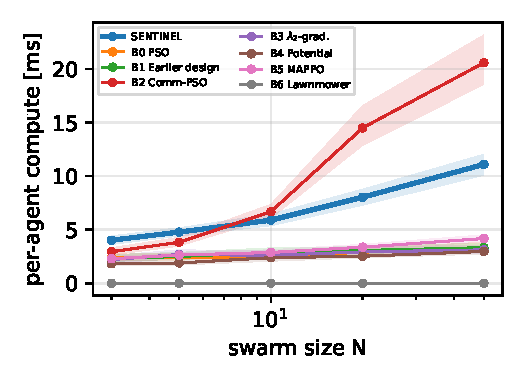
\includegraphics[width=\columnwidth]{figures/e1_compute_200m.pdf}
\caption{Per-agent planning time vs.\ swarm size on the 200\,m area (mean and 95\,\% CI over 30 seeds).}
\label{fig:compute}
\end{figure}

\subsection{Moving obstacles}\label{sec:eval:dynamic}
With 5 or 15 tall debris objects drifting through the area, blocking links and hiding victims
(Table~\ref{tab:e4}), SENTINEL keeps reporting 0.58 of the victims within 60\,s and remains
significantly better than all baselines (best baseline 0.48--0.51).
% generated by make_results.py -- do not edit by hand
\begin{table}[t]\centering\caption{Victims reported within 60 s with moving obstacles (urban, N=8). Mean over 30 seeds; best per column in bold; $^*$: differs from SENTINEL (paired Wilcoxon, Holm-corrected, $p<0.05$).}\label{tab:e4}
\setlength{\tabcolsep}{4pt}\begin{adjustbox}{max width=\columnwidth}\begin{tabular}{lccc}\toprule
Method & 0 moving & 5 moving & 15 moving \\\midrule
SENTINEL & \textbf{0.575} & \textbf{0.585} & \textbf{0.579} \\
B0 PSO & 0.453$^*$ & 0.481$^*$ & 0.460$^*$ \\
B1 Earlier design & 0.409$^*$ & 0.424$^*$ & 0.447$^*$ \\
B2 Comm-PSO & 0.468$^*$ & 0.489$^*$ & 0.509$^*$ \\
B3 $\lambda_2$-grad. & 0.475$^*$ & 0.479$^*$ & 0.487$^*$ \\
B4 Potential & 0.127$^*$ & 0.132$^*$ & 0.141$^*$ \\
B5 MAPPO & 0.396$^*$ & 0.449$^*$ & 0.431$^*$ \\
B6 Lawnmower & 0.421$^*$ & 0.443$^*$ & 0.425$^*$ \\
\bottomrule\end{tabular}\end{adjustbox}
\end{table}


\subsection{Detection uncertainty}\label{sec:eval:uncertainty}
We perturbed the calibrated detector model around its default: confidence noise
$\sigma\in\{0.04,0.08,0.15,0.25\}$, a weaker detector ($c_{\max}\in\{0.8,0.7\}$) and more frequent
false alarms. SENTINEL stays significantly ahead of B0 and B6 in all eight settings (0.45--0.81 vs.\
at most 0.59). Because the default false-alarm confidences rarely exceed the confirmation threshold,
we also ran a deliberately adverse case (Table~\ref{tab:e6c}): hot clutter that scores up to a mean of
0.55, the confidence noise applied to false alarms as well, and false alarms three times more
frequent. SENTINEL still reports 0.71--0.73 of the victims within 60\,s against at most 0.50 (B0), with
0.18 false confirmed entries per mission on average (B0: 0.29). Moving the SA band and the
confirmation threshold (0.3/0.6 to 0.4/0.85) changes the on-time share between 0.64 and 0.74 without
producing false confirmations.
% generated by make_results.py -- do not edit by hand
\begin{table}[t]\centering\caption{Victims reported within 60 s with hot-clutter false alarms (urban, N=8, $\sigma$=0.15). Mean over 30 seeds; best per column in bold; $^*$: differs from SENTINEL (paired Wilcoxon, Holm-corrected, $p<0.05$).}\label{tab:e6c}
\setlength{\tabcolsep}{4pt}\begin{adjustbox}{max width=\columnwidth}\begin{tabular}{lcccc}\toprule
Method & $\mu_{\mathrm{fp}}$=0.22, $r$=0.1 & $\mu_{\mathrm{fp}}$=0.4, $r$=0.1 & $\mu_{\mathrm{fp}}$=0.55, $r$=0.1 & $\mu_{\mathrm{fp}}$=0.55, $r$=0.3 \\\midrule
SENTINEL & \textbf{0.731} & \textbf{0.719} & \textbf{0.724} & \textbf{0.709} \\
B0 PSO & 0.501$^*$ & 0.491$^*$ & 0.500$^*$ & 0.493$^*$ \\
B6 Lawnmower & 0.480$^*$ & 0.480$^*$ & 0.479$^*$ & 0.481$^*$ \\
no SA & 0.715 & 0.693 & 0.708 & 0.668 \\
no fusion & 0.672$^*$ & 0.655$^*$ & 0.676$^*$ & 0.691 \\
\bottomrule\end{tabular}\end{adjustbox}
\end{table}


\subsection{What produces the gains}\label{sec:eval:ablation}
Table~\ref{tab:e7} removes one component at a time. Two components matter. First, multi-view fusion:
removing it reduces on-time reports significantly (urban, $N=8$: 0.519 vs.\ 0.575), and in the dense
swarm of Table~\ref{tab:e11_dense_diag} the corroborative rule is decisive (0.809, against 0.656 with
plain naive-Bayes fusion and 0.720 for B0). Second, the delivery trigger: Fig.~\ref{fig:thold} sweeps
$T_h$; in the severe channel with eight UAVs, delivering immediately ($T_h=0$) raises the on-time
share from 0.388 (never delivering) to 0.497 and lowers the 90th-percentile latency from 97\,s to
34\,s, while the total share of reported victims stays at 0.50. In the urban channel the same trend is
present but not significant. The remaining components (outage-based instead of distance-based spring,
LMST instead of nearest-neighbour preserved set, information-dependent tension, projection) do not
change the outcome significantly, and the SA flank is not significant in the tuned configuration.
These mechanisms act only during the short delivery tethers; we regard them as the safety layer
examined next, not as the source of the performance gains. Keeping the swarm connected at all times
(SENTINEL-strict) lowers on-time reporting to 0.03--0.13.
% generated by make_results.py -- do not edit by hand
\begin{table}[t]\centering\caption{Ablation: victims reported within 60 s (400 m, Poisson failures). Mean over 30 seeds; best per column in bold; $^*$: differs from SENTINEL (paired Wilcoxon, Holm-corrected, $p<0.05$).}\label{tab:e7}
\setlength{\tabcolsep}{4pt}\begin{adjustbox}{max width=\columnwidth}\begin{tabular}{lcccc}\toprule
Method & severe, N=4 & severe, N=8 & urban, N=4 & urban, N=8 \\\midrule
SENTINEL & \textbf{0.212} & 0.433 & 0.313 & 0.575 \\
SENTINEL-strict & 0.029$^*$ & 0.061$^*$ & 0.064$^*$ & 0.131$^*$ \\
distance spring & 0.200 & 0.433 & 0.307 & 0.561 \\
NN set & \textbf{0.212} & 0.433 & 0.313 & 0.573 \\
no info. tension & 0.211 & 0.433 & 0.312 & 0.572 \\
no projection & 0.200 & 0.435 & 0.308 & 0.545 \\
no SA & 0.189 & \textbf{0.455} & \textbf{0.316} & \textbf{0.583} \\
no fusion & 0.187 & 0.408 & 0.288 & 0.519$^*$ \\
naive-Bayes fusion & 0.167 & 0.439 & 0.300 & 0.540 \\
\bottomrule\end{tabular}\end{adjustbox}
\end{table}

% generated by make_results.py -- do not edit by hand
\begin{table}[t]\centering\caption{Dense swarm (200 m, N=50): victims reported within 60 s; ablations of SENTINEL and baselines with its fusion rule (same seeds). Mean over 30 seeds; best in bold; $^*$: differs from SENTINEL (paired Wilcoxon, Holm-corrected, $p<0.05$).}\label{tab:e11_dense_diag}
\setlength{\tabcolsep}{4pt}\begin{adjustbox}{max width=\columnwidth}\begin{tabular}{lc}\toprule
Method & 50 \\\midrule
SENTINEL & 0.809 \\
B0 PSO & 0.720$^*$ \\
no SA & 0.799 \\
no fusion & 0.740$^*$ \\
naive-Bayes fusion & 0.656$^*$ \\
no SA, no fusion & 0.719$^*$ \\
B0 + fusion & 0.815 \\
B1 + fusion & 0.819 \\
B2 + fusion & 0.833 \\
B3 + fusion & 0.815 \\
B4 + fusion & \textbf{0.865$^*$} \\
B5 + fusion & 0.819 \\
B6 + fusion & 0.849 \\
\bottomrule\end{tabular}\end{adjustbox}
\end{table}

\begin{figure}[t]\centering
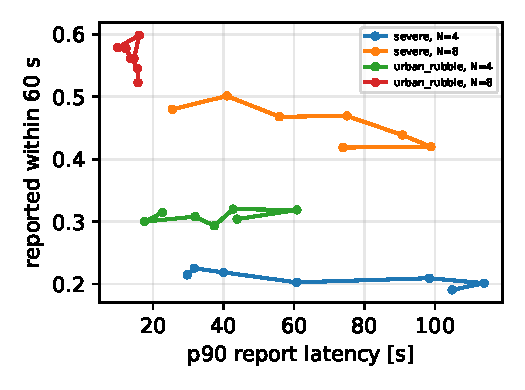
\includegraphics[width=\columnwidth]{figures/e10_thold_tradeoff.pdf}
\caption{Delivery trigger $T_h\in\{0,15,30,60,120,240,\infty\}$: on-time share vs.\ 90th-percentile
report latency for four regimes (each point: mean of 30 seeds).}
\label{fig:thold}
\end{figure}

\subsection{Link preservation during delivery}\label{sec:eval:safety}
Proposition~\ref{prop:link} is a one-step guarantee for feasible steps. Over all experiments we
counted the tethered, mutually preserved links that were reliable before a step and unreliable after
it: 15 violations in 436\,057 link-steps ($3.4\times10^{-5}$); with the swarm tethered at all times
(SENTINEL-strict) the rate is $2.6\times10^{-3}$. The residual violations come from steps where the
constraint was infeasible and the UAV hovered (Section~\ref{sec:proj}). Information loss did not vary
consistently with $T_h$ at the failure rates studied (at most 6.2\,\% in any cell), so the exposure
bound of Proposition~\ref{prop:exposure} could not be confirmed or refuted empirically; it remains a
design guarantee.

\subsection{Cross-validation in PX4/Gazebo and the earlier scenario}\label{sec:eval:sitl}
To check that the fast simulator does not depend on idealised flight, we flew SENTINEL and B0 with
three PX4 x500 multicopters in Gazebo Harmonic on the same three 100\,m areas and seeds (300\,s,
crash of one UAV at 150\,s), with the same agent code, tuned values, channel emulation and detector
model. The share of reported victims (SENTINEL 0.53 vs.\ 0.60 in the fast simulator; B0 0.60 vs.\
0.62), the packet delivery ratio (0.79--0.81 vs.\ 0.80--0.83) and the connected fraction agree within
0.07; coverage of SENTINEL is higher in SITL (0.99 vs.\ 0.83). With three seeds this is a consistency
check rather than a statistical comparison. Finally, re-running the scenario of the earlier SENTINEL design
(25\,m area, three UAVs, one crash) shows that it cannot separate the methods: the
area is far smaller than the radio range, every method stays connected throughout, and 64--69\,\% of
the victims are reported by all of them. The remaining victims are either buried or so close to
another victim (4--5\,m) that their reports merge (7.8--11\,\% of confirmations), which is a
limitation of the association gate rather than of connectivity.
